%!TEX root = ../../../main.tex
%%---------------------------------------------------------------------------
\section{Flow control overview}
\label{sec:rc_flow_control}
%%---------------------------------------------------------------------------
The overall system flow is explained in figure \ref{fig:overall_system_diagram}. This section deals with the system encapsulated as the robot cell. The overall states of the  robot cell is as shown in figure \ref{fig:rc_main_state}. This describes the four waiting states and the actions performed when switching state.
	
	\begin{figure}[H]
		\centering
	    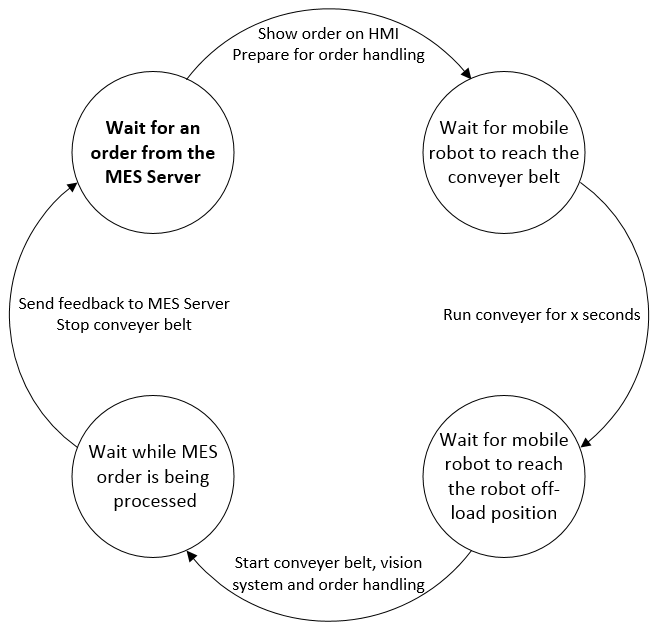
\includegraphics[width=0.85\textwidth]{rc_main_state_diagram}
	    \caption{Overall state diagram of the robot cell}
		\label{fig:rc_main_state}
	\end{figure}
	
Figure \ref{fig:rc_nodes} shows the elements that the robot cell consists of and the connection between them. The center is the main node which acts as the application and main point of the brick sorting program. 

	\begin{figure}[H]
		\centering
	    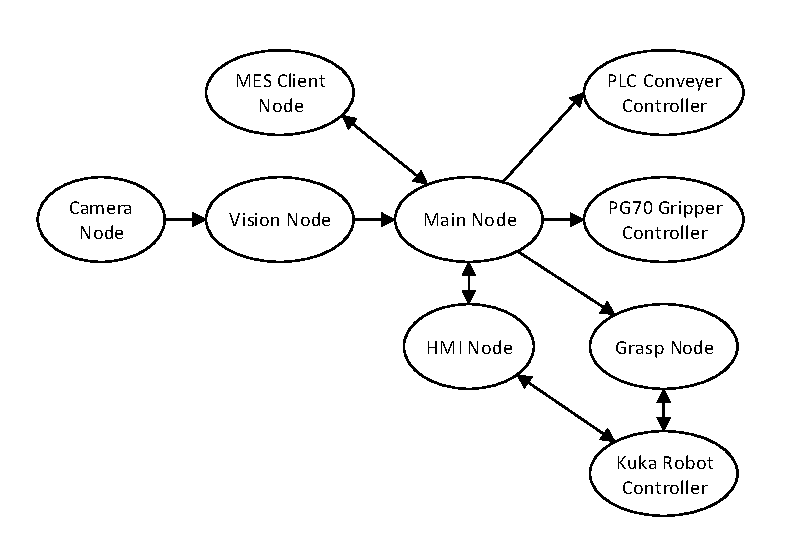
\includegraphics[width=0.8\textwidth]{rc_nodes}
	    \caption{ROS Node structure}
		\label{fig:rc_nodes}
	\end{figure}
	
The next sections cover the details of some of these nodes.
	